%************************************************
\chapter{The data}\label{ch:mathtest} % $\mathbb{ZNR}$
%************************************************
Night-time lights data are released by NASA and the EOG project of the Colorado School of Mines. Data is published with different time windows, namely nightly, monthly and yearly.
As I will illustrate in this chapter, the data need to be cleaned before being used, and the two sources use different data cleaning algorithms. Nasa has a faster publishing speed. In fact, data is published each night just over an hour after the satellite took the imagery. On the other hand, the EOG data, from the analysis I have carried out, implements a more effective data cleaning algorithm. Moreover, NASA files are published in tiles, small portions of space that must be processed before they can be used. Each tile must be geolocalised in space according to the order in which the tile is positioned.

\section{Dealing with satellite data}

Night-Time light data are distributed in georeferenced .tif images, which are images that contain map projection information, namely the coordinate reference system. 
Raster files are  $n \times k$  matrices that divide the observation surface into rectangular pixels.

\begin{figure}[h]
    \begin{center}
    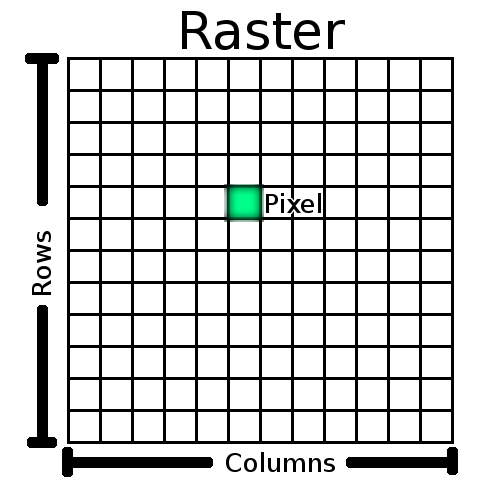
\includegraphics[width=7cm]{images/raster_dataset.png}
    \end{center}
    \caption{Raster representation - Source: Qgis Docs}
\end{figure}


With night-time lights, each cell of the raster matrix contains the reflectance measured in that portion of the Earth.
Depending on the sensor's technology mounted on the satellite, the pixels will capture smaller portions of the globe, producing higher resolution images. 

Given the circular motion of the satellite orbit, the resolution is measured in arc/seconds. Regarding the two main technologies in the night-time lights industry, the viirs sensor data has a resolution of 15 arc/seconds (circa 400 metres at the equator) while the previous DMSP sensor data is about 30 arc/seconds (circa 1000 metres at the equator). 
\begin{figure}[h]
    \begin{center}
    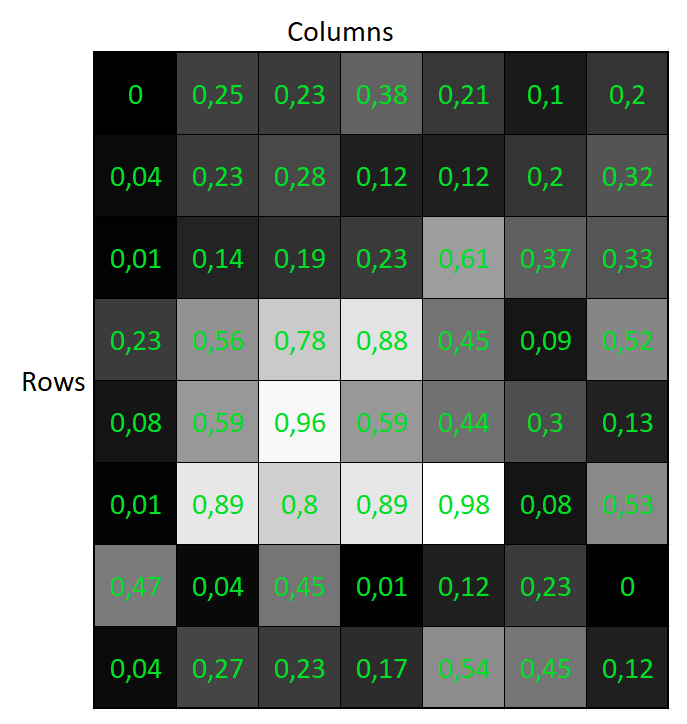
\includegraphics[width=7cm]{images/raster_night.png}
    \end{center}
    \caption{Night-time raster representation}
\end{figure}
The geographic reference system divides the Earth into 360 equal segments called degrees. Each degree contains 60 minutes and therefore 3600 seconds.
An arc-second is the geographical distance measured on the surface of the Earth after one second's rotation, or 1/3600th of a degree.
At the equator, one arc/second of latitude corresponds in metres to one arc/second of longitude. However, the further one moves towards the poles, the equivalent of one arc/second in longitude decreases.
  
In order to perform 'zonal statistics', i.e. statistics of delimited areas of the globe, it is necessary to delimit the raster files with another file that contains georeferenced information about geographical boundaries. For this purpose, most of the time, Shapefiles or GeoJson are used, which are called "polygon files", which are files containing information about the boundaries of the geographical regions to be studied. As with raster files, polygon files can also have different resolutions. In this thesis, I will use the data with the highest possible resolution distributed by GADM.
\begin{figure}[h]
    \begin{center}
    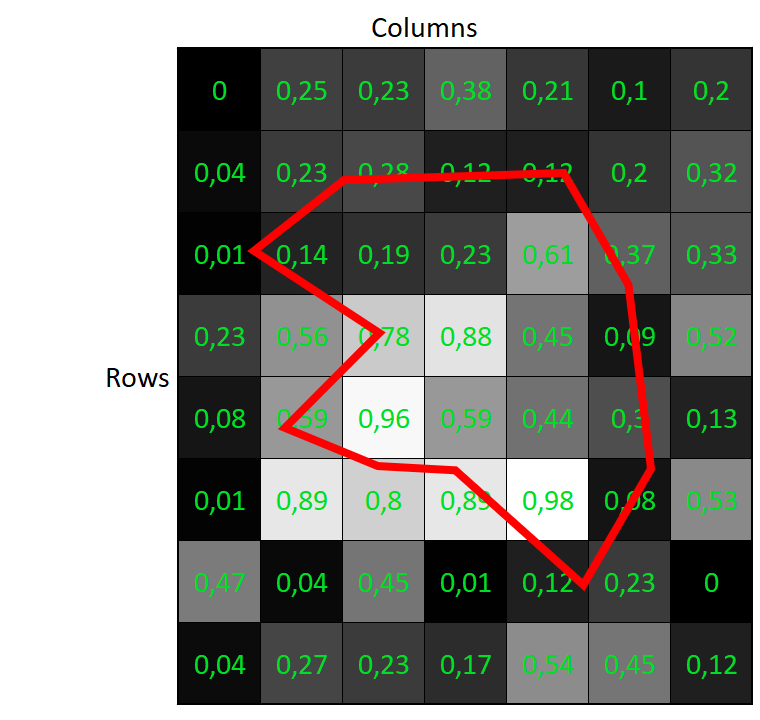
\includegraphics[width=7cm]{images/raster_night_cover.png}
    \end{center}
    \caption{Night-time lights extraction process representation}
\end{figure}
Gadm is a free open access database of global administrative areas which produces the highest quality border files.
The geographical area to be studied is obtained from the intersection of the raster file and the polygon file. Then we can run statistical functions. In this thesis, I will make use of summation and spatial variance.

An important consideration must be made regarding the data extraction process. It is legitimate to ask how to deal with pixel values only partially contained within the geographical boundaries of interest. In this thesis, I will use the R package 'exactextractr', which is the most refined package for data extraction. This package, unlike the alternatives, extracts values by weighting them for effective coverage. 
A final note on the analysed data is the weight they occupy on the disk. An annual panel analysis of 11 years results in a data volume of around 120GB multiplied by 12 (i.e. around 1.5 terabytes) if the analysis is carried out with monthly data. 

\section{Data problems}
Managing satellite data is complex. One of the difficulties is dealing with the some issues that without correction may give biased data. This is the reason why research on the best algorithms for cleaning and producing data does not stop and new types of algorithms are constantly updated. The three main problems we face are:
\begin{enumerate}
\item \textbf{Cloud Coverage:} As argued earlier, one of the many purposes of night lights was to study the presence of cloud bodies. It is therefore not surprising that, if only interested in the dynamics of the emitted illumination, the complete or partial overlay of clouds may result in missing or dirty data. 
The data published by both NASA and EOG also include detailed information on the areas where clouds were present at the time of the survey. It is up to the researcher to choose whether the amount of daily data without cloud cover is sufficient for his purpose. 
An alternative that solves or improves the problem is to use information of the areas covered by clouds from other periods. To do this, the time window of analysis must be increased. Several algorithms have been developed to aggregate daily data into monthly or annual surveys. 
The operation is not complex and works as follows, given several daily surveys in one layer of raster information and another layer with the different cloud cover of the respective days, the algorithm takes only the values of the non-covered or partially covered areas and through a specific statistical function (mean or median most of the time) reconstructs a complete image.
Although very rare, a particular area may be covered for a whole month by clouds that prevent a correct representation of the actual light emitted. For this reason, it is necessary to consider the percentage of cloud-free observations of that month. Otherwise, data would be biased and annual aggregates may have to be used.
\item \textbf{Natural lights:} when measuring night-time lights, the presence of natural lights is a problem. Natural lights include sunlight, moonlight, reflections, fires, burning biomass and other ephemeral events.
Dealing with these problems is much more complex than cloud coverage. Different strategies have been adopted, and achieving the highest possible quality is still far away. 
The first of the strategies adopted in the field is cleaning through data aggregation, as seen above. This is because some of these natural lights have a seasonal nature. For instance, as is shown in the following images, some areas of northern Europe in the summer months suffer from overexposure to light at night, and the resulting images have entire areas burnt out. This kind of problem can be solved satisfactorily by aggregating an entire year's daily images.
On the other hand, other natural light sources have no seasonal character, namely, among the others, burning biomass and reflections. In this case, the remote sensing literature has treated these problems as outliers and tried to propose some solutions. For instance, the first version of EOG used a histogram-based technique in which the tails were cut off. This data was further cleaned by eliminating background noise by identifying a minimum threshold in the neighbourhood of each pixel.
\item \textbf{Stray Lights:} In optics, stray lights are defined as instrumental noise in optical systems due to unwanted light, namely reflections or lens imperfections. Again, various algorithms have been created to deal with this issue. EOG publishes two types of data, "vcm" is the raw non-stray light corrected data, while "vcmsl" is the clean data.
\end{enumerate}
The data I will use in this thesis are those of EOG project. In the last years they adopted three versions of the cleaning algorithm, V1.0, V2.0, V2.1 which have gradually become more and more sophisticated in handling the issues mentioned above.
Version 2.0 of the algorithm updates the threshold detection used to eliminate the light background in a sophisticated manner. Without intending to be exhaustive, the new algorithm calculates the median of the maximum values of the multiyear time series, weighted for cloud-free observations. A scattergram of the observations is then created by plotting the percentage of cloud free versus threshold, and a gamma curve was fit to lie above the scattergram noise levels. From this gamma curve, we obtain the threshold for each observation of the globe for each cloud-coverage level.
Finally, a significant problem was caused by the Aurora Borealis. Increasing the threshold too much would have resulted in a significant loss of information in other areas of the globe. Therefore, a 'manual' approach was adopted by overlaying a layer on the residual noise in the north and south aurora zones.
As mentioned earlier, although these algorithms constitute state of the art in the field, they have not yet achieved very high levels of quality. When analysing the data, I found some anomalies. If I extract the maximum observable values, I find very high values in Russia in the middle of nature that seems to be the effect of gas flaring, a phenomenon due to the high quantity of natural gas processing plants in the region.
Although \citeauthor{elvidge2021annual} claim in the version 2.0 algorithm paper \citep{elvidge2021annual} to have dealt adequately with outliers, they actually don't. Data still suffer of pixels 200 times brighter than the most populated capitals in the world and this is the result of median outlier removal that has only success with seasonal phenomena. These outliers are few, but they take high values and the sum extraction process risks of resulting in biased data. In the following sections, I will try to deal with this problem.
\section{Outliers}
A quick analysis of the data shows that the brightness of a city of 500,000 to 1 million inhabitants reaches maximum values of between 100 and 250 light units. The city of Milan, one of the brightest places in Italy, reaches maximum values of 130/140 lit in the centre and around 200 at its airports. Other European cities have similar characteristics, with London reaching maximums of 200/240 lit in the area around Piccadilly and Oxford Circus, and Paris and Rome reaching values of no more than 120/150 lit in the centre. American cities that are generally considered brighter reach higher values. The brightest point in New York is the block between the Rockefeller center and Time Square and reaches a peak of about 420 lit. These values are in line with the largest world capitals, which are generally considered bright. Dubai is generally less bright than New York except for the pixel containing the Burj Kalifa, the world's tallest skyscraper, which reaches brightness levels of over 500 litres. Asian cities are all in line with New York and in the vast majority of cases emit lower peaks of light. Hong Kong, for example, does not exceed 220 litres, Shenzen 100, and is very similar to Milan, while Tokyo, the brightest of the Asian cities, barely exceeds 400 litres.

The brightest city in the world is undoubtedly Las Vegas, the average values in the city centre being around 1,000 litres for an area absolutely out of the average of 11 square kilometres with these light levels. In addition, the pixel containing The Luxor Hotel & Casino is a real outlier with an emitted light level of 6000 lit. The reason is quickly stated, the pyramid-shaped hotel emits a beam of light at its apex that is directed towards the sky. As I will illustrate in the following lines, I will consider this type of light among the outliers and it will be ignored in the subsequent analysis. 

Although, as reported earlier, the EOG project claims to have handled outliers from an in-depth analysis of the data it appears that some outliers still remain. Russia is one of the countries whose images suffer most from this problem. Looking at night-time images of Russia, multiple pixels with values that are totally out of scale can be seen. For instance, pixels with values around 10000 lit in the middle of nowhere, tens of kilometres away from population centres.
Studying point by point, I found two interesting phenomena. The first is that indeed Russia is dotted with gas flares, which are fields with vents burning day and night. The second is that, surprisingly, these flames are exceeded in light output by sheds in the middle of the steppe. After an initial moment of bewilderment, I cross-referenced OpenStreetMap data and some Google search, and I discovered that such sheds are indeed technologically advanced greenhouses. Russia's solid agricultural vocation, with limited energy costs, has led to the flourishing of greenhouses heated and illuminated by thousands, but perhaps millions, of light bulbs turned on day and night. 
\begin{figure}
    \centering
    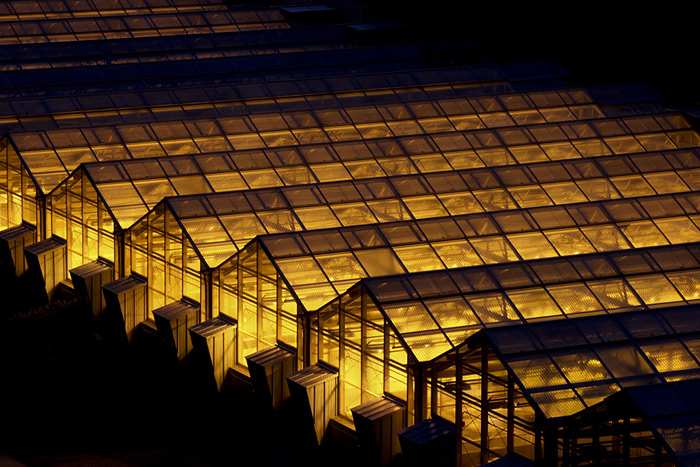
\includegraphics[width=7.5cm]{images/greenhousesatnight.jpg}
    \caption{Greenhouse}
    \label{fig:my_label}
\end{figure}
These kind of greenhouses are entirely transparent to maximise the amount of light reaching the plants, and the combination with a very high amount of light makes them some of the brightest places on Earth. This kind of greenhouse can also be found outside Russia. All countries with high latitudes need to compensate for the lack of light, especially during the winter. This is because, in such latitudes, the indoor greenhouse cultivation system does not have enough natural sunlight. To my knowledge, greenhouses never appear in the literature even though it is a significant problem that needs to be addressed. In 2021, the total light emitted by Russia cleaned by these two phenomena was about 40 per cent less than the un-cleaned figure. A vast difference that, however, seems to be so invasive for Russia only. In other European countries, this phenomenon is much more limited. In Italy, for example, no such outlier can be observed, not even in Spain, France and Germany. The only exception is Holland, which has several greenhouses of the same Russian technology, albeit in smaller proportions.
As far as night fires are concerned, on the other hand, I found no outliers in Europe with the same Russian magnitude. On the contrary north African countries, endowed with well-known oil deposits, are full of them. 

Dealing with these outliers raises some critical economic questions. Greenhouses and gas flares enter directly into the GDP count. It is therefore questionable whether it is correct to eliminate or keep them. However, it is unrealistic to think that a pipeline vent in Siberia that emits as much light as an average Italian city has the same impact on GDP. Therefore, I decided to carry on cleaning the data from outliers but keep the original data, which will be compared on the following pages. 

\subsection{Outlier Removal strategies}

Several strategies are adopted to deal with outliers:
\begin{enumerate}
    \item Spatial correction: the algorithm checks each pixel and compares it with the surrounding area, usually 3x3 or 5x5 pixels. If the value of the pixel is several orders of magnitude higher than the average of the surrounding area, the pixel is recognised as an outlier and is removed
    \item Statistical correction: a predetermined percentile of the data distribution is removed. (For data from Russia, tests suggest the removal of the 0.001 tail)
    \item Manual correction: By looking at the values of cities and the central infrastructure of a country (airports, first of all), it is possible to derive a maximum threshold beyond which all other data are outliers. As far as Russia is concerned, the maximum value observed in cities is less than 500, while all values above are greenhouses or gas flares.
\end{enumerate}

For reasons of computational power, in this thesis, I will use the second and third approaches. It appears to be sufficient with a more rude data outlier removal. Moreover, power and RAM at a server level are required to manipulate this type of data.
%*****************************************
%*****************************************
%*****************************************
%*****************************************
%*****************************************
